\section{Deep Gated Network : Gating Experiments}
An important upshot of duality is that the gates can be treated as masks, which can then be held externally and applied to the network of weights. This decoupling of gates and weights is achieved by the deep gated network (DGN) setup \cite{npk}.
The DGN setup is useful to characterise the role played by the gates in a `standalone' manner. In particular, the DGN enables one to separately study various kinds of gates such as random gates (of a randomly initialised network), semi-learnt gates (sampled at an intermediate epoch during training), and learnt gates (sampled from a fully trained network).  
\subsection{DGN Setup}
\FloatBarrier
\begin{figure}[h]
\resizebox{\columnwidth}{!}{
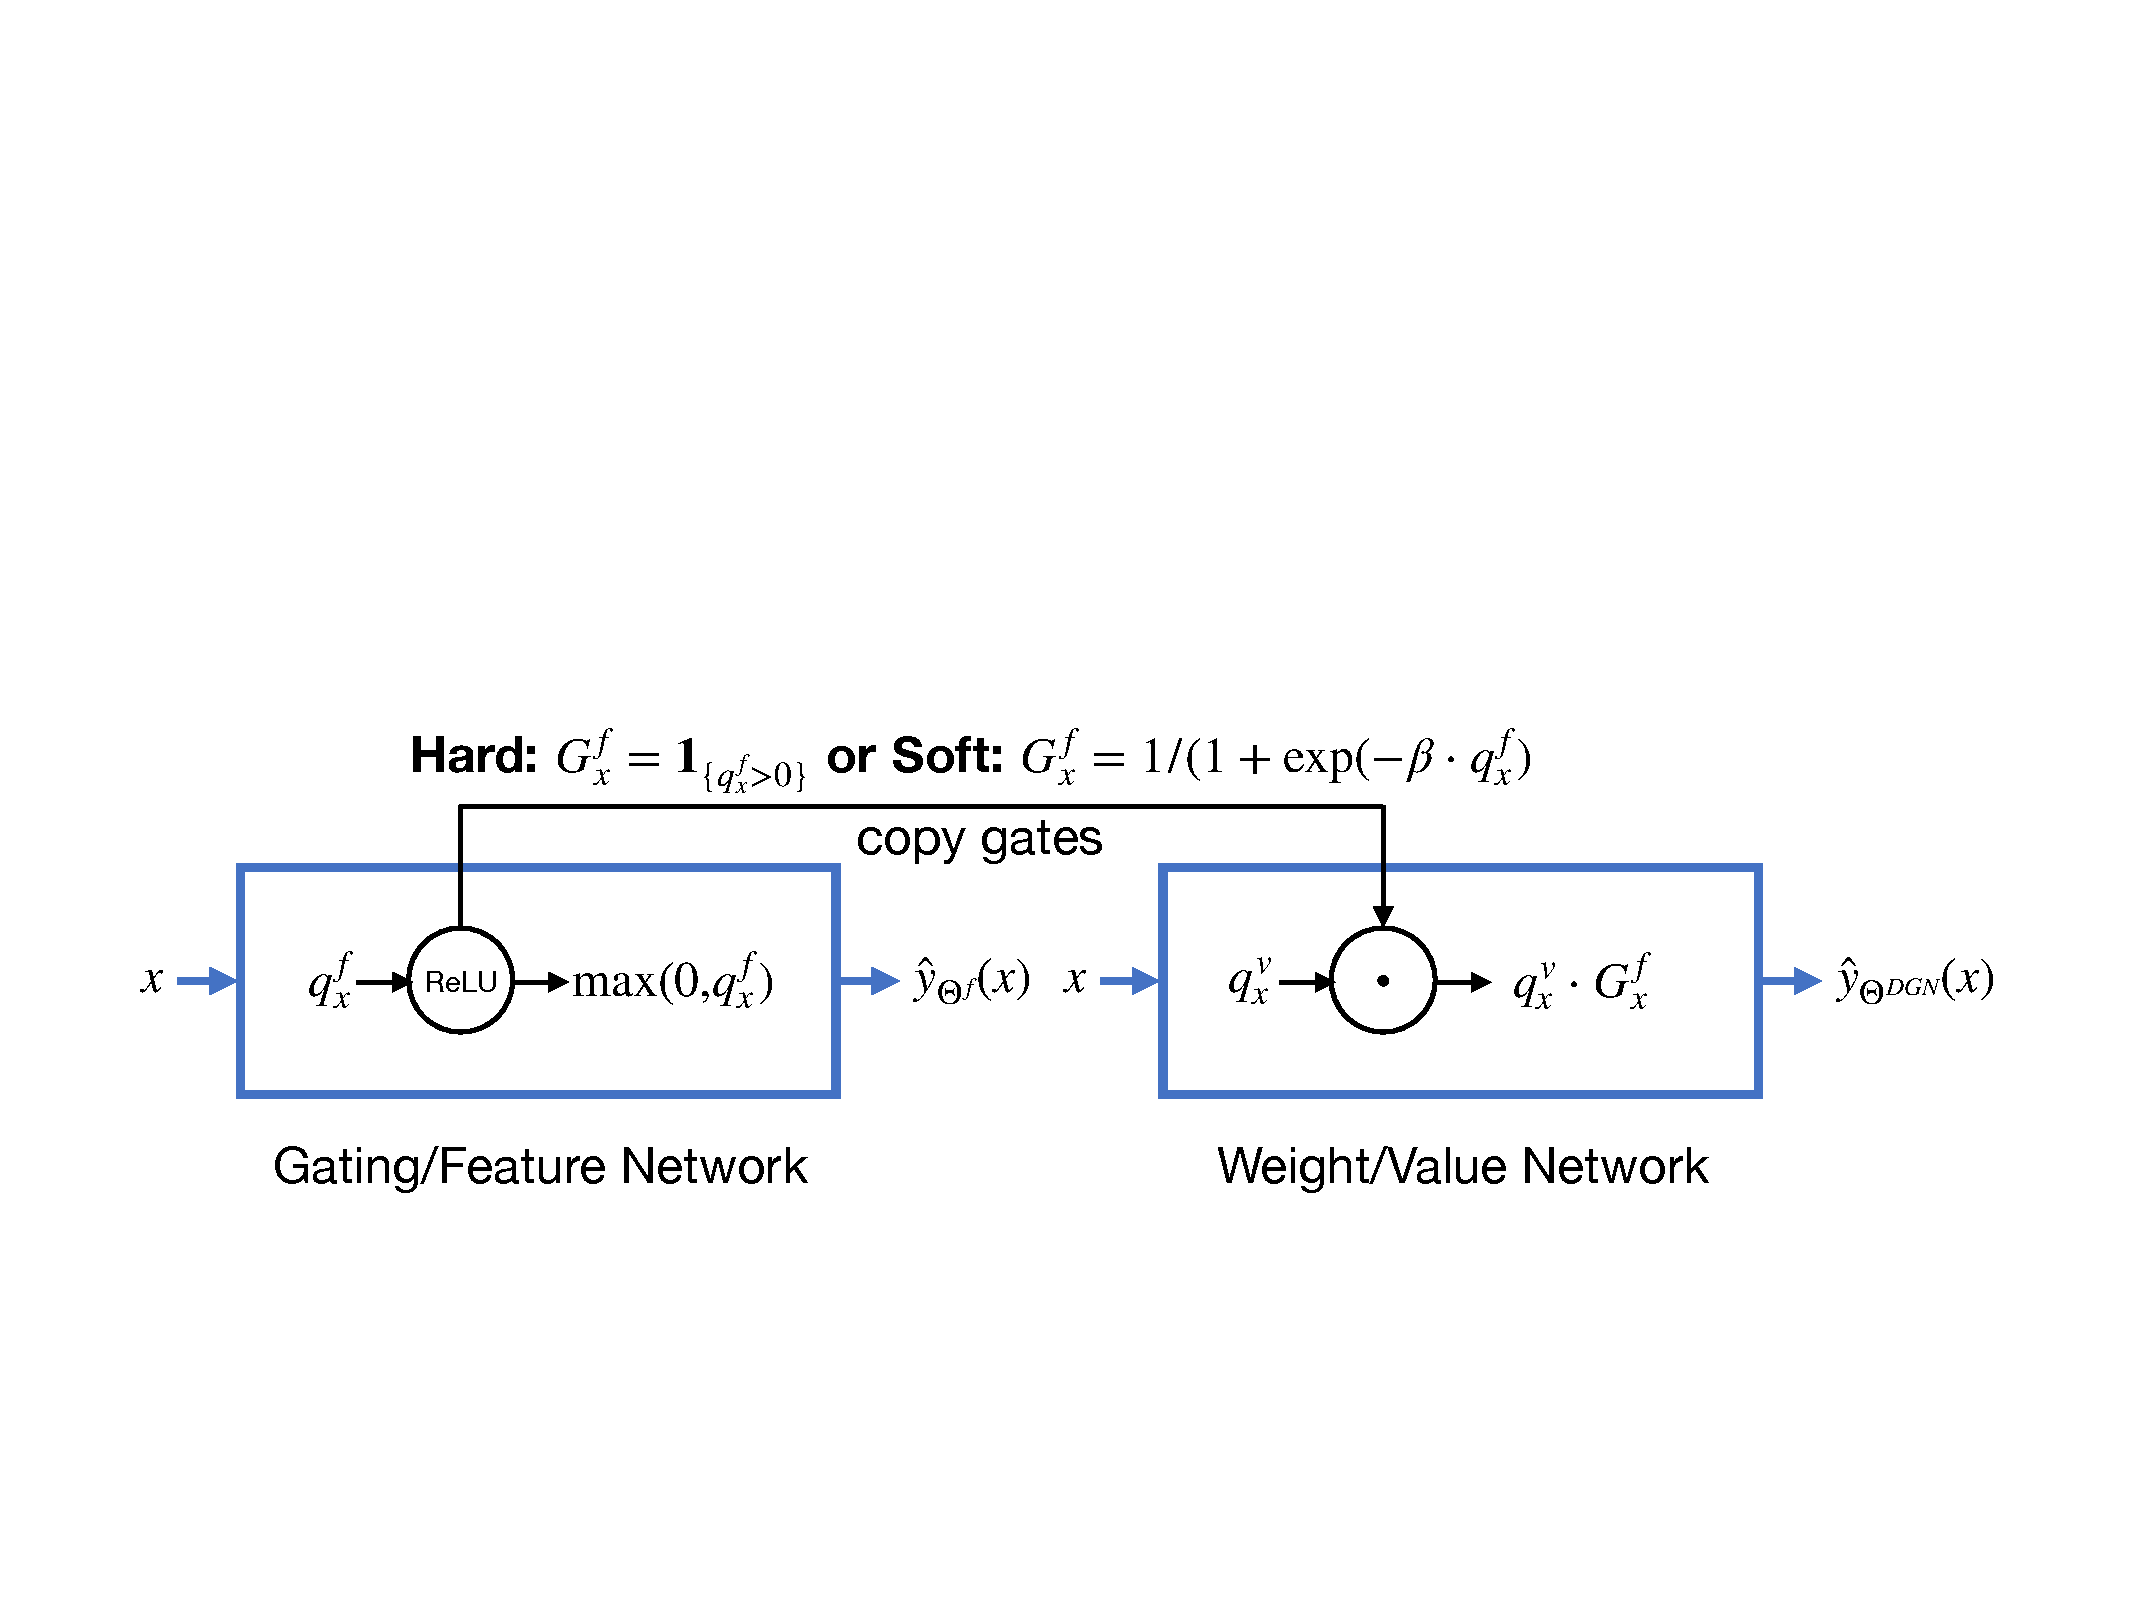
\includegraphics[scale=0.3]{figs/dgn-simple.pdf}
}
\end{figure}
 The DGN has two networks namely the \emph{feature network} parameterised by $\Tf\in\R^{d^{\text{f}}_{\text{net}}}$ which holds the NPFs (i.e., the gating information) and a \emph{value network} parameterised by $\Tv\in\R^{d^{\text{v}}_{\text{net}}}$ which holds the NPV.  The combined parameterisation is denoted by $\Theta^{\text{DGN}}=(\Tf,\Tv)\in \R^{d^{\text{f}}_{\text{net}}+d^{\text{v}}_{\text{net}}}$.  Thus the learning problem in the DGN is $\hat{y}_{\Tdgn}(x)=\ip{\phi_{x,\Tf},v_{\Tv}}$. 
\subsection{$\text{NTK}=\text{NTK}^{\text{fixed-gate}}+\text{NTK}^{\text{gate-learn}}$}
In a DGN, the gradient $\nabla_{\Tdgn}\hat{y}_{\Tdgn}(x)$ has two components i.e., $\nabla_{\Tdgn}\hat{y}_{\Tdgn}(x)=\left(\nabla_{\Tf}\hat{y}_{\Tdgn}(x),\nabla_{\Tv}\hat{y}_{\Tdgn}(x) \right)$, where $\nabla_{\Tf}\hat{y}_{\Tdgn}(x)$ flows through the feature network, and $\nabla_{\Tv}\hat{y}_{\Tdgn}(x)$ flows through the value network. This gives rise to the relation $\text{NTK}=\text{NTK}^{\text{fixed-gate}}+\text{NTK}^{\text{gate-learn}}$, where $\text{NTK}^{\text{fixed-gate}}$ is the kernel corresponding to learning of the weights with the gates fixed and $\text{NTK}^{\text{gate-learn}}$ is the kernel corresponding to learning of gates themselves. 
\begin{proposition}\label{prop:ntks} Let $K_{\Tdgn}$ be the NTK matrix of the DGN, then $K_{\Tdgn}=\kv_{\Tdgn}+\kf_{\Tdgn}$, with
\resizebox{\columnwidth}{!}{
\begin{tabular}{|p{2cm}|p{6cm}|}\hline
NTK & $K(x,x')=\ip{\nabla\hat{y}(x),\nabla\hat{y}(x')}$\\\hline
$\text{NTK}^{\text{gate-learn}}$ & $\kf(x,x')=\ip{ \nabla_{\Tf}\hat{y}(x), \nabla_{\Tf}\hat{y}(x') }$\\\hline
$\text{NTK}^{\text{fixed-gate}}$ & $\kv(x,x')=\ip{ \nabla_{\Tv}\hat{y}(x), \nabla_{\Tv}\hat{y}(x') }$\\\hline
\end{tabular}
}
\end{proposition}
\subsection{DGN Regimes}
% Here the gates/`active sub-networks' are held in the feature network and are then used in the value network.
\begin{definition}\label{rm:regime}The DGN has $\mathbf{4}$ \textbf{regimes} namely \emph{decoupled learning} (DL), \emph{fixed learnt} (FL), \emph{fixed random-dependent initialisation} (FR-DI) and \emph{fixed random-independent initialisation} (FR-II). 
In all the regimes $\hat{y}_{\Tdgn}$ is the output, and $\Tv_0$ is always initialised at random and is \emph{trainable}. However, the regimes differ based on i) trainability of $\Tf$, ii) initialisation $\Tf_0$ as described below.\\
\begin{tabular}{|l|p{6cm}|}\hline
DL               & $\Tf$ is trainable, and $\Tf_0$ and $\Tv_0$ are random and statistically independent,  $\beta>0$.\\\hline
FL               & $\Tf$ is non-trainable, and $\Tf_0$ is pre-trained;  $\Tv_0$ is statistically independent of $\Tf_0$. \\\hline
FR-II            & $\Tf$ is non-trainable, and $\Tf_0$ and $\Tv_0$ are random and statistically independent.\\\hline
FR-DI   &  $\Tf$ is non-trainable, and $\Tf_0=\Tv_0$.\\\hline
\end{tabular}
\end{definition}
The flexibility in a DGN is that  a) $\Tf$ can be trainable/non-trainable and b) $\Tf_0$ can be random or pre-trained using $\hat{y}_{\Tg}$ as the output (\Cref{rm:regime}). By using the DGN setup we can study the role of gates by comparing (a) learnable (DL) vs fixed gates (FL, FR-DI, FR-II), (b) random (FR-DI, FR-II) vs learnt gates (FL) and (c) dependent (FR-DI) vs independent initialisations (FR-II). In the DL regime `soft-ReLU' is chosen to enable gradient flow through the feature network.
%\end{comment}

\textbf{Remark:} In the case of fixed regimes, $\kf=0$. 
